\documentclass{beamer}

\usepackage[utf8]{inputenc}
\usetheme{default}

\title{First-arrival traveltime tomography based on the adjoint-state method}

\AtBeginSubsection[]
 {
  \begin{frame}<beamer>{Outline}
   \tableofcontents[currentsection,currentsubsection]   
  \end{frame}
 }

\begin{document}
 
 \begin{frame}
  \titlepage
 \end{frame}

 \begin{frame}{Outline}
  \tableofcontents
 \end{frame}
 
 \section{Introduction}
 
 \subsection{Motivation}
 
 \begin{frame}{Motivation}
  
 \end{frame}

 \section{Theory}
 
 \begin{frame}{Gradient of the misfit function}
  \begin{itemize}
   \item Misfit function for a single-shot
   \begin{equation}
    J({c}) = \frac{1}{2}\int_{\partial\Omega}d\boldsymbol{r}|T({c},\boldsymbol{r}) - T_{obs}(\boldsymbol{r})|^2
   \end{equation}
   \item Gradient method
   \begin{equation}
    {c}_{n+1} = {c}_n - \alpha_n\nabla J({c}_n),
   \end{equation}
    where $\alpha$ is a positive scalar.
  \end{itemize}
 \end{frame}

 \begin{frame}{Gradient of the misfit function}
  \begin{itemize}
   \item Extended misfit function
   \begin{eqnarray}
    L({c},t,\lambda) = &&\frac{1}{2}\int_{\partial\Omega}d\boldsymbol{r}|t(\boldsymbol{r}) - T_{obs}(\boldsymbol{r})|^2 \nonumber \\
    - &&\frac{1}{2}\int_\Omega d\boldsymbol{x}\lambda(\boldsymbol{x})\bigg(|\nabla t(\boldsymbol{x})|^2 - \frac{1}{{c}(\boldsymbol{x})^2}\bigg)
   \end{eqnarray}
   \item for $t(\boldsymbol{x}) = T(\boldsymbol{x})$
   \begin{equation}
    L({c},T,\lambda) = J({c})
   \end{equation}
  \end{itemize}
 \end{frame}
 
 \section{Implementation}
 
 \subsection{Fast-sweeping method}
 
 \begin{frame}{Fast-sweeping method}
  \begin{itemize}
   \item Eikonal equation
   \begin{equation}
    |\nabla T(\boldsymbol{x})|^2 =  \frac{1}{c^2(\boldsymbol{x})}
   \end{equation}
   
   \begin{equation}
    T(\boldsymbol{x}_s) = 0
   \end{equation}
   \item Adjoint-state system
   \begin{equation}
    \Lambda(\boldsymbol{r})\boldsymbol{n}(\boldsymbol{r})\cdot\nabla T(\boldsymbol{r}) = T(\boldsymbol{r}) - T_{obs}(\boldsymbol{r})
   \end{equation}
   
   \begin{equation}
    \nabla\cdot\Lambda(\boldsymbol{x})\nabla T(\boldsymbol{x}) = 0
   \end{equation}
  \end{itemize}
 \end{frame}

 \begin{frame}{Fast-sweeping method}
  \begin{itemize}
   \item Godunov upwind FD scheme
   \begin{equation}
    \bigg[\frac{(T(\boldsymbol{x})-T(\boldsymbol{x})^{xmin})^+}{\triangle x}\bigg]^2 + \bigg[\frac{(T(\boldsymbol{x})-T(\boldsymbol{x})^{zmin})^+}{\triangle z}\bigg]^2 = \frac{1}{c^2(\boldsymbol{x})} \nonumber
   \end{equation}
  \end{itemize}
 \end{frame}
 
 \begin{frame}{Fast-sweeping method}
  \begin{itemize}
   \item Initialize $T(\boldsymbol{x}_s) = 0$ and assing very large positive values to the rest of the grid points.
   
   \item Update grid points with Gauss-Seidel and keep the smallest value between the old and the calculated. $min(T_{old},T^*)$
  
   \item Check the convergence $||T^{n+1} - T^n||_{L1} \leq \varepsilon$ for $\varepsilon > 0$
   \end{itemize}
 \end{frame}
 
 \begin{frame}{Fast-sweeping method}
  \begin{itemize}
   \item Adjoint-state
   \begin{equation}
    \frac{\partial}{\partial x}(a\lambda) + \frac{\partial}{\partial z}(b\lambda) = 0
   \end{equation}
   where $a = \partial t(x,z)/\partial x$ and $b = \partial t(x,z)/\partial z$
   
   \item $a$ and $b$ values
   \begin{equation}
    a_{i + \frac{1}{2},j} = \frac{t_{i+1,j} - t_{i,j}}{\triangle x}, \qquad a_{i - \frac{1}{2},j} = \frac{t_{i,j} - t_{i-1,j}}{\triangle x}
   \end{equation}
   
   \begin{equation}
    b_{i,j+\frac{1}{2}} = \frac{t_{i,j+1} - t_{i,j}}{\triangle z}, \qquad b_{i,j - \frac{1}{2}} = \frac{t_{i,j} - t_{i,j-1}}{\triangle z}
   \end{equation}
  \end{itemize}
 \end{frame}

 \begin{frame}
  \begin{itemize}
   \item Introducing the notations:
   \begin{equation}
    a^\pm_{i + \frac{1}{2},j} = \frac{a_{i + \frac{1}{2},j} \pm |a_{i + \frac{1}{2},j}|}{2}
   \end{equation}

   \begin{equation}
    a^\pm_{i - \frac{1}{2},j} = \frac{a_{i - \frac{1}{2},j} \pm |a_{i - \frac{1}{2},j}|}{2}
   \end{equation}
 
   \begin{equation}
    b^\pm_{i,j+\frac{1}{2}} = \frac{b_{i,j+\frac{1}{2}} \pm |b_{i,j+\frac{1}{2}}|}{2}
   \end{equation}
   
   \begin{equation}
    b^\pm_{i,j-\frac{1}{2}} = \frac{b_{i,j-\frac{1}{2}} \pm |b_{i,j-\frac{1}{2}}|}{2}
   \end{equation}


   
   
  \end{itemize} 
 \end{frame}

 
 
 \section{Exemples}
 
 \subsection{Gradient calculation}
 
 \begin{frame}{Gradient calculation}
  \begin{itemize}
   \item Constant vertical-gradient velocity model with a velocity anomaly.
   
   \item 2km in depth and 7.5km laterally. 12.5m by 12.5 grid size.
   
   \item 600 sources and 600 receivers for each source.
  \end{itemize}
 \end{frame}
 
 \begin{frame}{Fast Sweeping Method}
  \centering
  \begin{figure}
   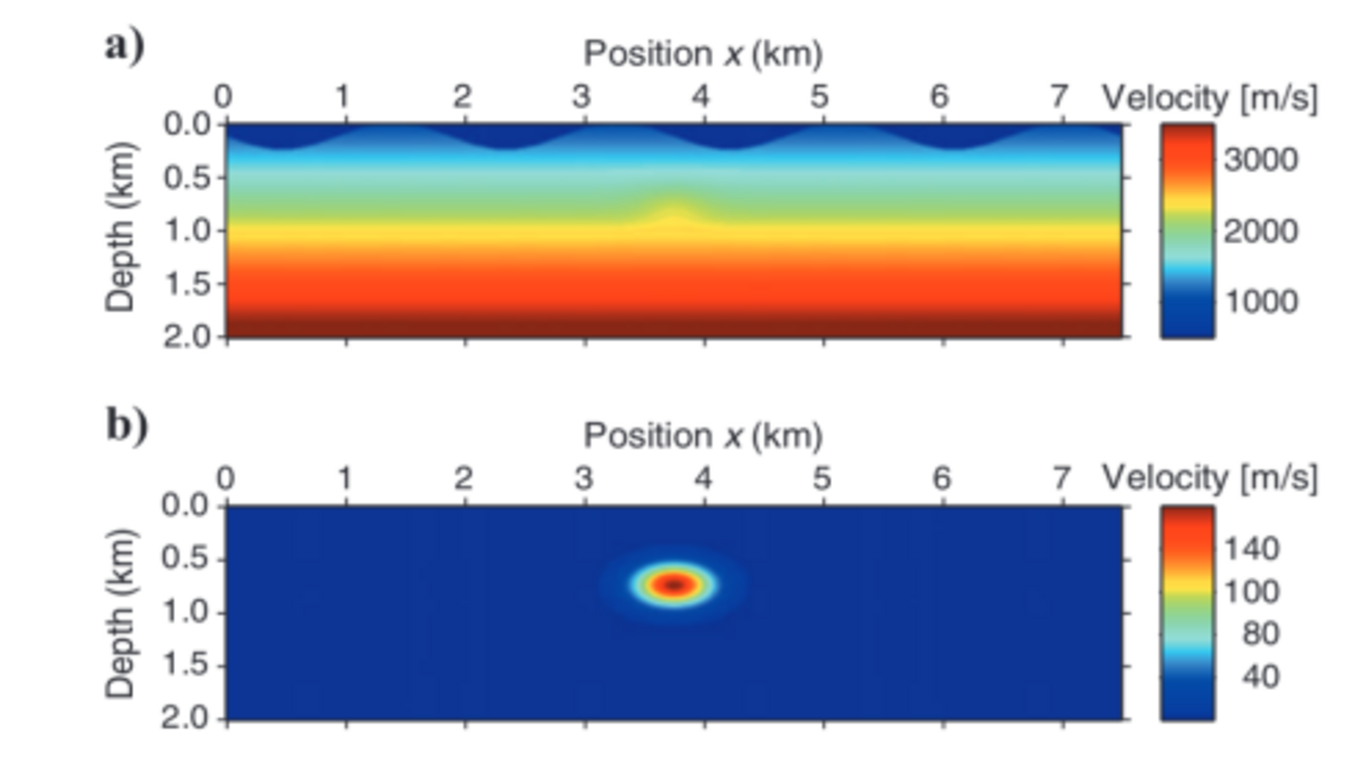
\includegraphics[width=8.5cm,height=7cm]{figuras/imag1.png}
  \end{figure}
 \end{frame}

 \begin{frame}{Fast Sweeping Method}
  \centering
  \begin{figure}
   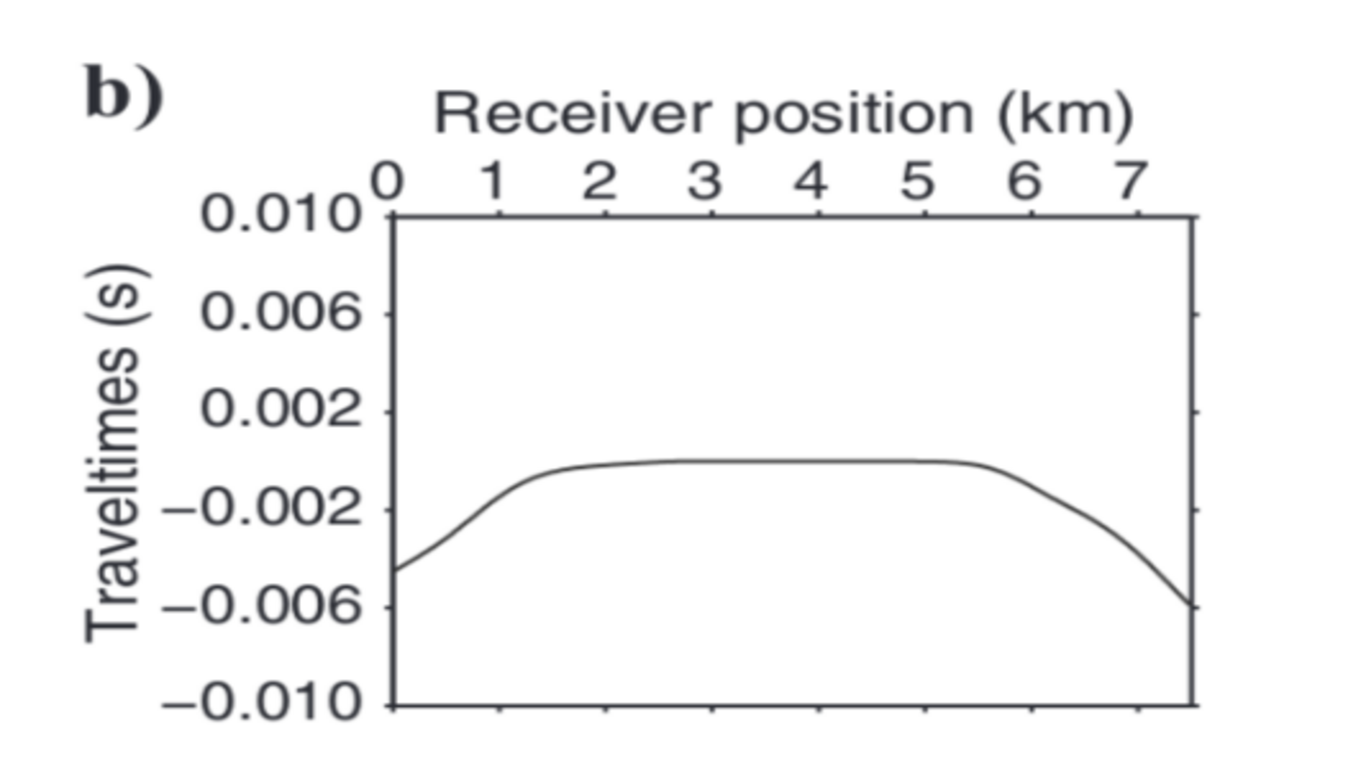
\includegraphics[width=8.5cm,height=5cm]{figuras/imag2.png}
  \end{figure}
 \end{frame}
 
 \begin{frame}{Fast Sweeping Method}
  \centering
  \begin{figure}
   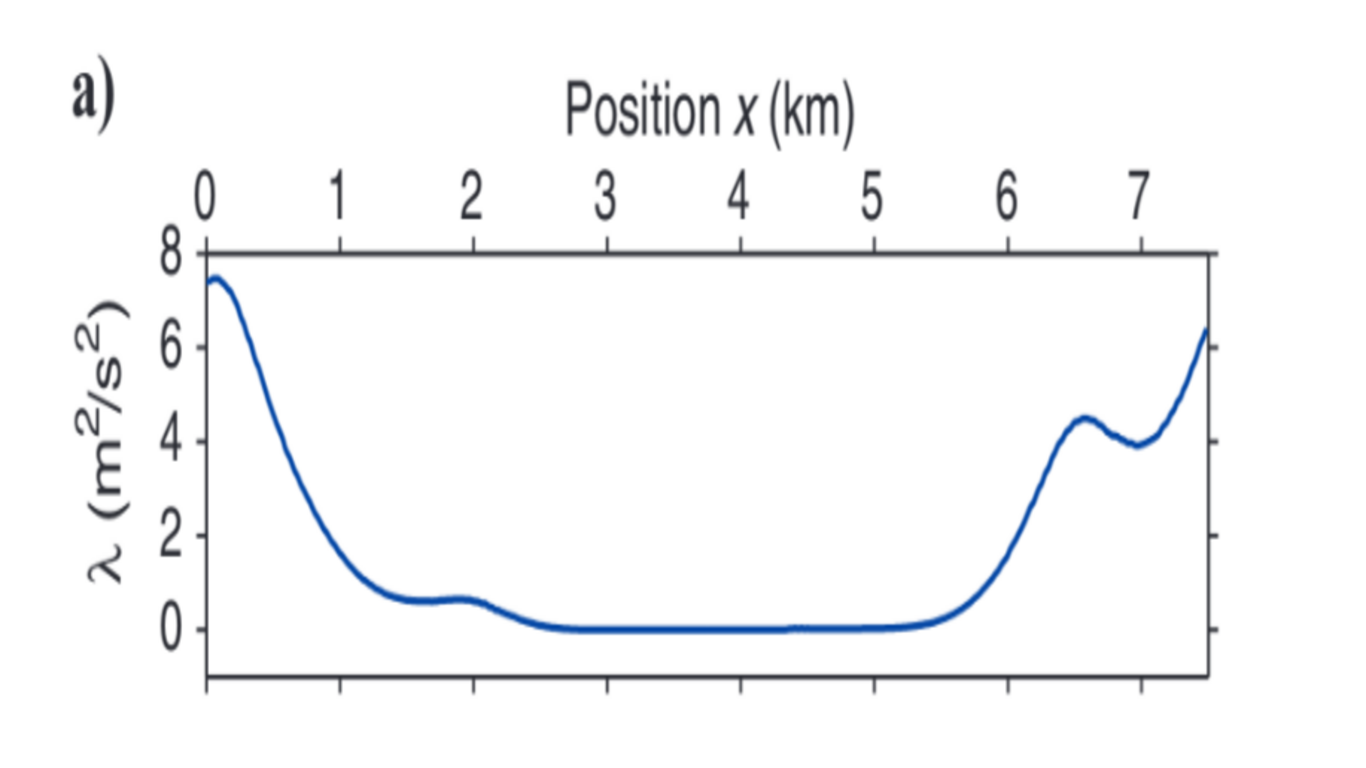
\includegraphics[width=8.5cm,height=4cm]{figuras/imag3.png}
  \end{figure}
 \end{frame}
 
 \begin{frame}{Fast Sweeping Method}
  \centering
  \begin{figure}
   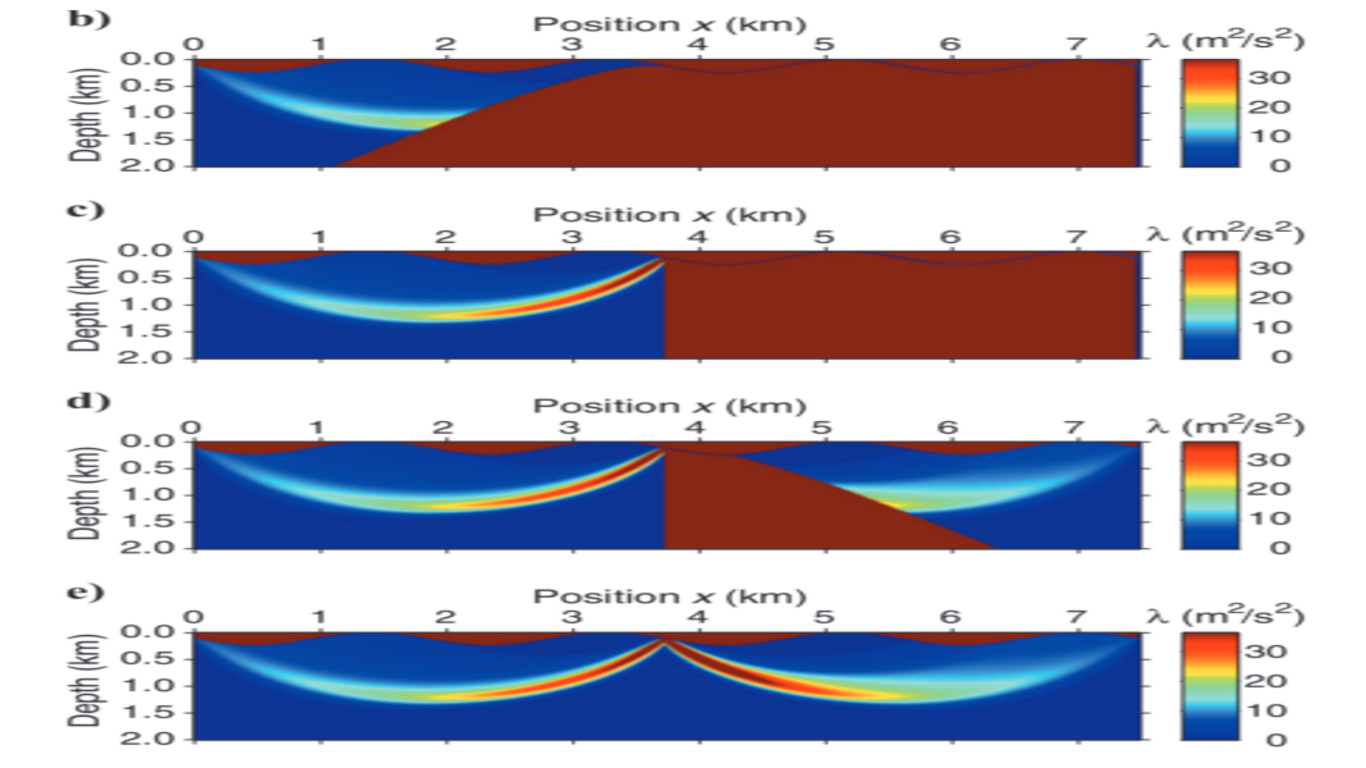
\includegraphics[width=7cm,height=7cm]{figuras/imag4.png}
  \end{figure}
 \end{frame}

 \begin{frame}{Fast Sweeping Method}
  \centering
  \begin{figure}
   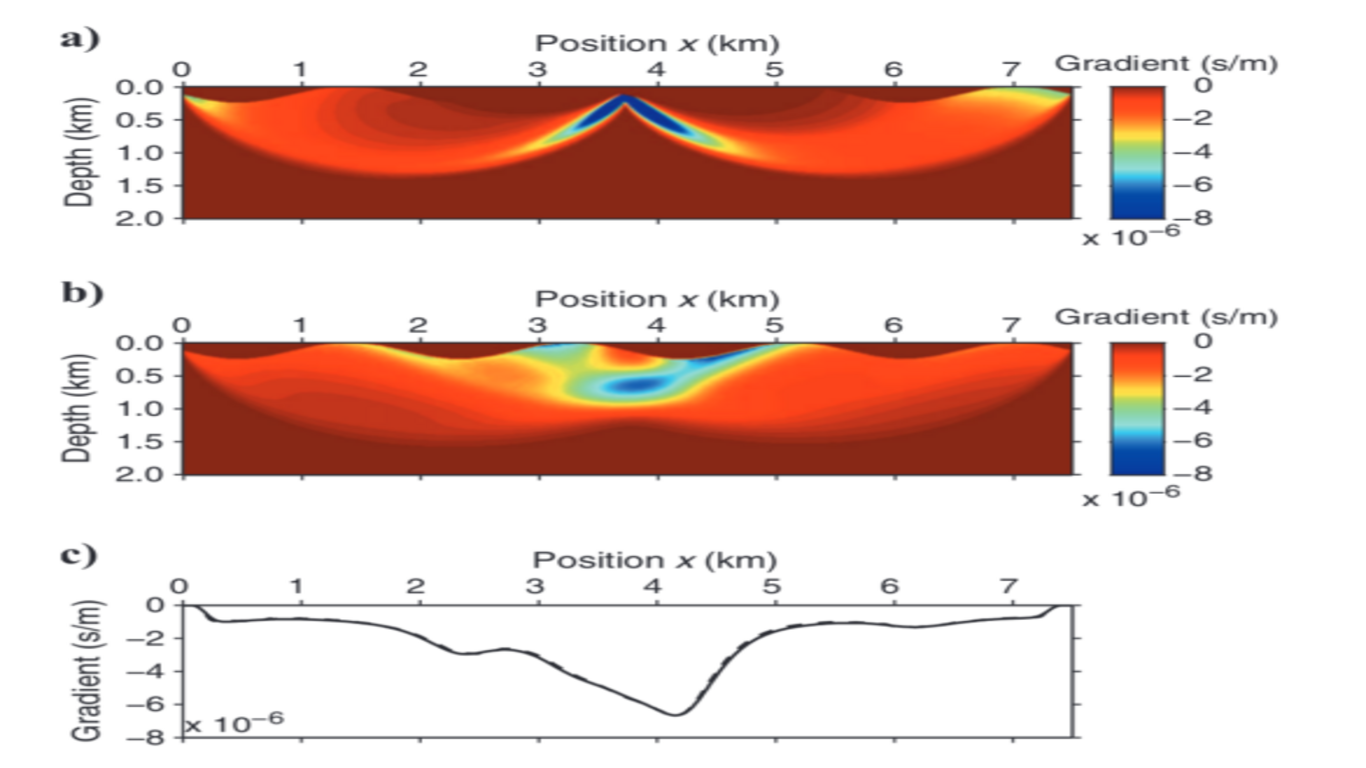
\includegraphics[width=7.5cm,height=7cm]{figuras/imag5.png}
  \end{figure}
 \end{frame}
 

\end{document}
